\documentclass{article}
\usepackage{float}
\usepackage{graphicx} 
\providecommand{\tightlist}{%
  \setlength{\itemsep}{0pt}\setlength{\parskip}{0pt}} 
\title{Computer Programming HW1: Turtle Edge Printer}

\author{B07202020\\
NTUEE/NTUPhys\\
Hao-Chien Wang}

\begin{document}
\maketitle
The goal of this program is to read an image, find the edge of the
image, and print it with the Turtle module. Several images are provided
to test. You can also use your own image.

\section{Instruction}

There are four parameters available for the user in the beginning of the
script:
\begin{enumerate}
	\item \texttt{FIGURE\_PATH} : set the path to the image.
	\item \texttt{FILTER\_STRENGTH} : Specify the strength of the filter. Higer
value will make the filter discard the edges that are not so obvious.
And since the total amoun of the line being drawn affect the time needed
to print the picture, higher value also results in faster print.
	\item \texttt{FAST\_MODE} : Boolean. the width of the countour is usually
		larger than one pixel. If true, the \textit{contour of contour} will be
printed. Solid contour (made of a lot of lines) will be printed
otherwise. Usually increase the speed more than 10 times if enabled.
	\item \texttt{RESIZE\_RATIO} : Resize the image. \texttt{New\_size\ =\ old\_size\ /\ RESIZE\_RATIO}
\end{enumerate}

\section{Function description}

The description of each function is also written in the comments of the
script.

\subsection{Modules imported}

\begin{itemize}
\tightlist
\item
  PIL: module to read pictures into an array of RGB values
\item
  NUMPY: convenient to process big arrays
\item
  math: required for the \texttt{sqrt()} function
\item
  sys: required to clear the last line of input
\item
  turtle: output method
\end{itemize}

\subsection{Functions for Image Processing}

\begin{itemize}
\tightlist
\item
  \texttt{readImage(\ filePath,\ rerize\ =\ 1\ )}: Read image and
  transform it into a 3D ( height $\times$ width $\times$ RGB values ) numpy array.
  Receives the path to the picture, ratio to resize ( with default value
  1 ), and return a 3D numpy array.
\item
  \texttt{brightness\_of\_elements(\ imageArrayElement\ )}: formula to
  calculate luminance. Receives a 1x3 array consisting the RGB value of
  the pixel and return the luminance.
\item
  \texttt{brightness(\ imageArray\ )}: Apply the
  \texttt{brigntness\_of\_elements} function to every pixel elements.
\item
  \texttt{linify(\ imageArray,\ filterStrength,\ fastMode\ =\ False\ )}
  : use the Prewitt filter to find the edge. Receives the image array
  ,the filterStrength specifying the strength of the filter and a
  boolean to decide whether to enable fastMode. The function first apply
  the filter to each pixel and get \texttt{processedArray}. Then, it
  normalize the value of the array, and set the value above
  \texttt{filterStrength} to 1 and otherwise 0, which is the
  \texttt{finalArray}. Finally, the function results the
  \texttt{finalArray}.
\item
  \texttt{getLineFig(\ filePath,\ filterStrength,\ fastMode,\ resize\ =\ 1\ )}
  : encapsulation for functions processing the figure array. Receives
  the path to the image, filterStrength, fastMode (boolean) and resize
  ratio, call the functions above, then return the processed image
  array.
\end{itemize}

\subsection{Functions for Turtle Drawing}

\begin{itemize}
\tightlist
\item
  \texttt{goto(\ t,\ x,\ y\ )}: move the turtle without drawing
  anything. Receives the Turtle object and the target coordinates.
\item
  \texttt{draw(\ figurePath,\ filterStrength\ =\ 1.5,\ fastMode\ =\ False,\ resize\ =\ 1,\ wait\ =\ True\ )}
  : encapsulation for drawing methods. Receives the path to the image,
  \texttt{filterStrength} (default value 1.5), fastMode (default value
  \texttt{False}), resize ratio, and a boolean \texttt{wait}(default
  value \texttt{True})specifying whether to wait after finishing the
  job. It also show the progress in the console. It will keep refreshing
  the same line, but this feature might not work in every machine.
\end{itemize}

\section{Examples}

\begin{figure}[H]
\centering
\includegraphics[width=\textwidth]{flower.bmp}
\caption{\texttt{flower.bmp}: The original image.}
\end{figure} 

\begin{figure}[H]
\centering
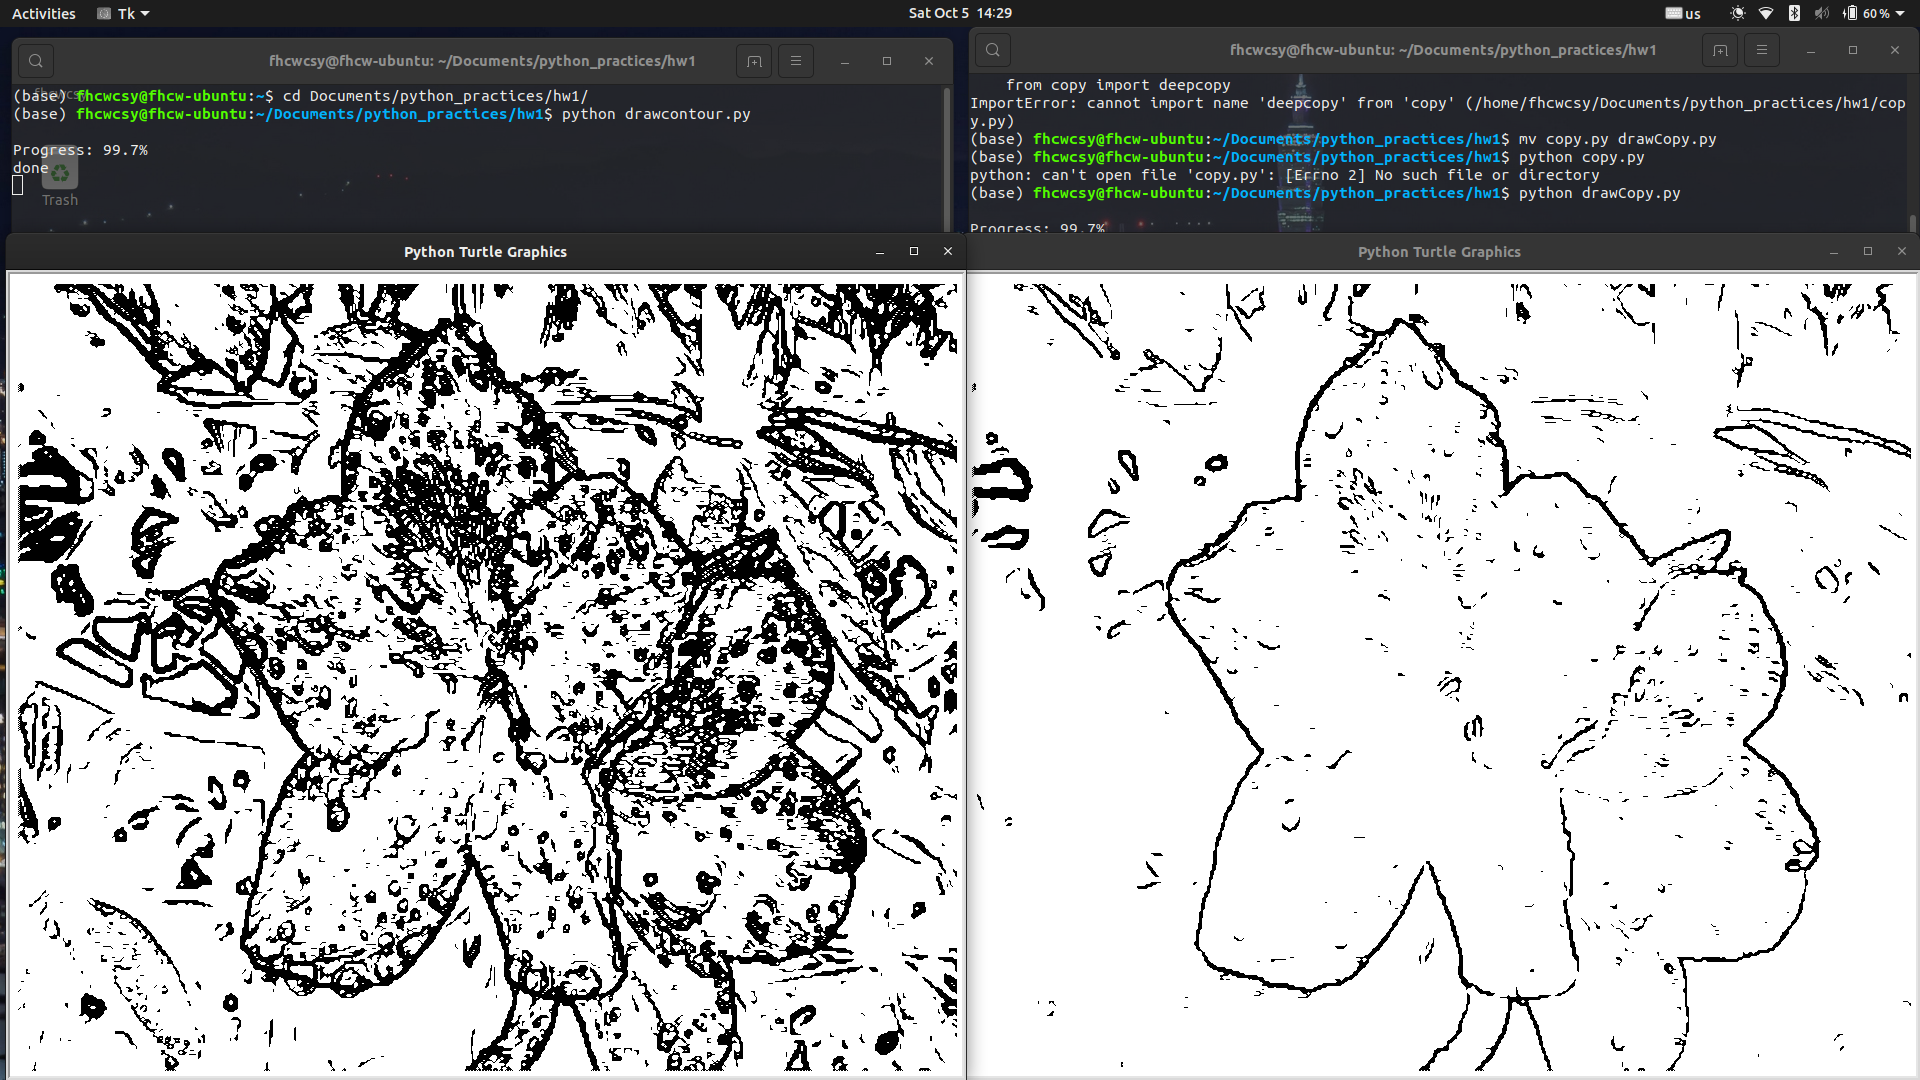
\includegraphics[width=\textwidth]{full.png}
\caption{Left: \texttt{FASTMODE = False, FILTER\_STRENGTH = 0, RESIZE\_RATIO = 1}. Right: \texttt{FASTMODE = False, FILTER\_STRENGTH = 1, RESIZE\_RATIO = 1}}
\end{figure} 

\begin{figure}[H]
\centering
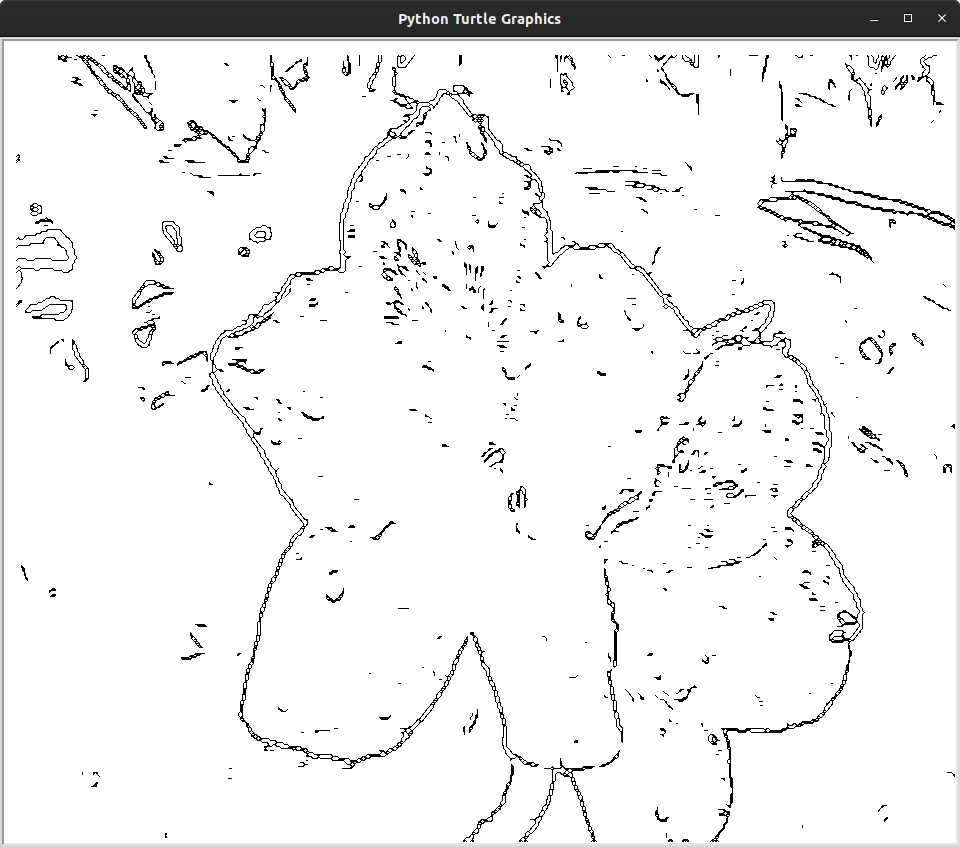
\includegraphics[width=\textwidth]{./simple1.png}
\caption{
\texttt{FASTMODE\ =\ True}, \texttt{FILTER\_STRENGTH\ =\ 1.5},
\texttt{RESIZE\_RATIO=1}
}
\end{figure} 

\begin{figure}[H]
\centering
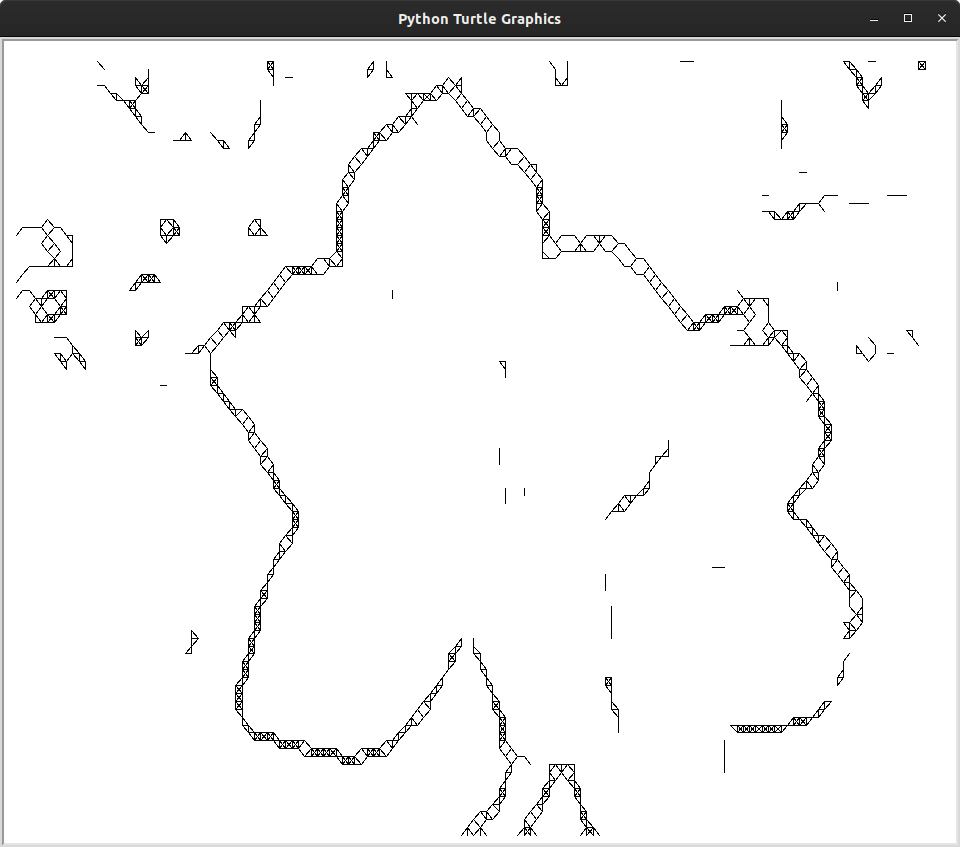
\includegraphics[width=\textwidth]{./simple4.png}
\caption{
\texttt{FASTMODE\ =\ True}, \texttt{FILTER\_STRENGTH\ =\ 1.5},
\texttt{RESIZE\_RATIO=4}
}
\end{figure} 

\begin{figure}[H]
\centering
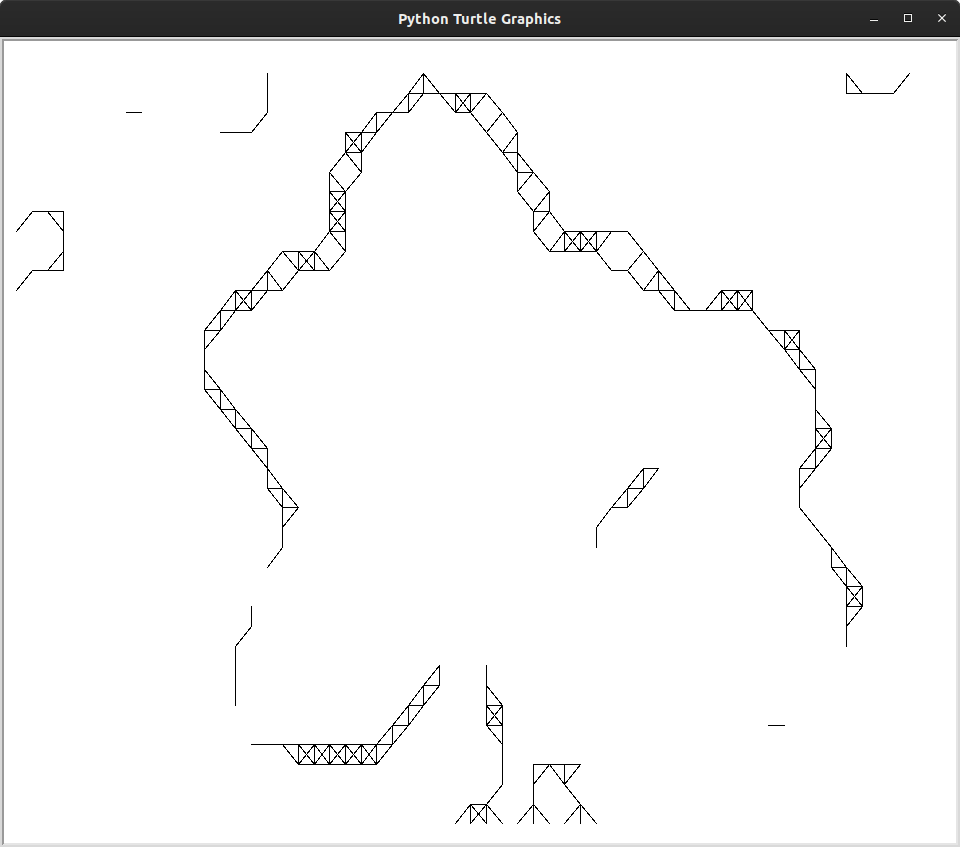
\includegraphics[width=\textwidth]{./simple10.png}
\caption{
\texttt{FASTMODE\ =\ True}, \texttt{FILTER\_STRENGTH\ =\ 1.5},
\texttt{RESIZE\_RATIO=10}
}
\end{figure} 

\end{document}
